\section{Introduction}
% \begin{figure}[t]
%     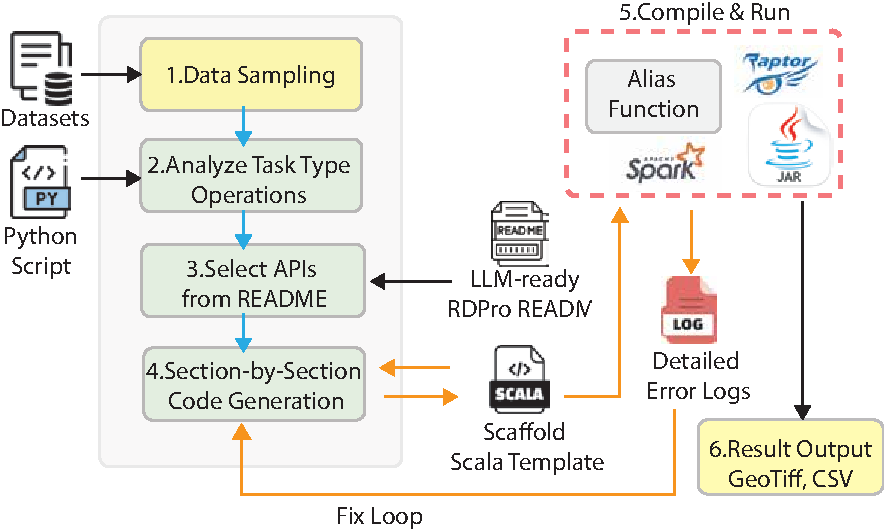
\includegraphics[width=\columnwidth]{figures/GRAIL.pdf}
%     \caption{GRAIL translation system overview}
%     \label{fig:grail}
% \end{figure}
% python -  scala
% nl - scala
% improve doc, log to LLM ready
% spark DAG
% evaluation: running time, token, data size

% 1- Importance of satellite data and difficulty in processing them using traditional methods.
Over the past decade, satellite data from missions such as Landsat, Sentinel, and MODIS has grown rapidly and become widely available for research on agriculture, land use, climate change, and disasters. However, the utilization of this data is limited by its massive volume. Most domain scientists use Python scripts that employ single-machine libraries, e.g., Rasterio and GeoPandas, which are great for prototyping and experimentation but do not scale to large parallel computation.


% 2- Scalable satellite proceessing systems and their limited use.

Recent systems such as Apache Sedona~\cite{yu2016demonstration}, GeoTrellis, and RDPro~\cite{shang2024rdpro} support scalable raster processing, but they require users to learn new frameworks, distributed computing concepts, and often Scala or Java, making them difficult for many data scientists to adopt. Recently, we worked closely with agronomists and hydrologists to port a complex model that predicts evapotranspiration (ET) maps to Apache Spark to support large-scale data~\cite{FieldSAT}. However, this approach is difficult to replicate due to the steep learning curve associated with Spark. Another approach is to develop a Python interface that wraps existing scalable functionality in RDPro but this requires substantial ongoing engineering effort and still requires additional learning.


% This creates a common problem to data scientists that they are often experts in their application domains, they may lack the expertise required to scale analytical pipelines. For example, agronomists studying crop yield estimation from satellite 
% data develop workflows that function 
% well on small study areas, but struggle to scale to larger regions 
% such as the entire state of California. One classical path forward 
% is to rewrite Python scripts into a scalable 
% pipeline~\cite{FieldSAT}, but this requires complex infrastructure 
% setup and forces domain scientists to manage execution environments with which they are unfamiliar. Another approach is to build a 
% Python interface that runs high-performance Scala code underneath, 
% but building and maintaining such a wrapper requires substantial 
% ongoing engineering effort.

% 3- Hint about LLMs and why they are not enough
Recent advances in LLMs offer an alternative path forward for making specialized libraries accessible to non-technical users. LLMs can now generate end-to-end programs from simple text descriptions~\cite{trummer2025generating, guo2024deepseek}, motivating this demo to explore translating data scientists' Python scripts, or even plain-text descriptions, directly into Scala code that runs on Spark~\cite{jin2025llms}. However, this approach presents three main challenges that are explored in this demo.
First, LLMs are well trained on common geospatial Python libraries such as GeoPandas and Rasterio, which have tons of examples used in training, but are less familiar with newer research libraries.
Second, code comments and README files are traditionally written for human consumption and may not provide the kind of information LLMs need~\cite{wijaya2025readme}.
Third, while much prior work studies code generation from text, less attention has been given to translating existing code across both programming languages and library ecosystems.


% making it possible to design systems where an AI agent 
% translate Python scripts into Scala, or generates Scala code directly 
% from a plain-text task description~\cite{jin2025llms}. Scientists can then continue working in a familiar way while benefiting from scalable distributed 
% execution underneath.

% However, applying LLMs to domain-specific libraries introduces its 
% own challenges. First, existing documentation is written for human 
% readers and often lacks sufficient examples or uses outdated API 
% references, making it difficult for LLMs to infer correct 
% usage~\cite{wijaya2025readme}. 
% Second, LLMs tend to default to general-purpose libraries they have 
% seen frequently during training, such as GDAL or standard Python 
% raster tools such as Rasterio, rather than adopting the terminology and patterns of a specialized library like RDPro. To address this, we focus on 
% making RDPro itself LLM-ready, rather than retraining a new model. 
% Since RDPro is a domain-specific geospatial library with limited 
% training data exposure, it is more practical to guide an existing 
% capable model through well-structured documentation and targeted 
% library modifications.

% 4- Hint about the proposed system and the code generation part
This paper presents GRAIL, a system that we developed to demonstrate and study how LLMs can be used with newly developed libraries that are still under development and do not have the advantage of being used in training.
Rather than focusing on the LLM side, we study how to make the library itself, RDPro~\cite{shang2024rdpro} in our case, LLM-ready so that it can work with existing agents and code generators.
GRAIL builds an agentic pipeline using LangGraph that is tailored for satellite data analysis.
It starts with analyzing the task in-hand, whether a Python script or a textual description, and then follows with a planning phase that uses a scaffold that guides the planning phase. After that, it generates the code section-by-section and finalizes with a validation and repair phase to produce the final code.

% 5- The library extensions that we added
In addition to the agent-based code generation, we also extend the RDPro library itself with three new ideas and test their effect on the correctness and quality of code generation.
First, we develop specialized documentation that is targeted towards LLMs rather than humans. They add more details and instructions that are specifically useful for LLM-based code generation.
Second, we extended the code itself with \emph{alias functions} that provide multiple entry points to the same functionality but with common standard terminology that the LLM is familiar with, e.g., using function names and signatures popular with other raster-based libraries.
Finally, we extend error messages to be more verbose and enrich them with instructions on how to fix the error. These detailed error instructions are designed so that a code generator can use as feedback to fix the code on the next iteration.


% GRAIL implements this as a structured agentic pipeline built on 
% LangGraph, where each stage is an explicit graph node with defined inputs and contractual outputs. With the help of a more LLM-ready library design, users can 
% either upload an existing Python script or describe their task in 
% natural language, and the system generates the corresponding Scala 
% program. This paper demonstrates the system through several example scenarios and different datasets.
%The remainder of this paper is organized as follows. Section~\ref{sec:system} provides the detailed GRAIL translation pipeline. 
%Section~\ref{sec:mod} describes
%three modifications to the RDPro codebase that improve LLM-generated 
%code reliability, covering structured documentation, alias functions, 
%and enhanced error messages. Section~\ref{sec:demo} demonstrates 
%use cases.
 %Then, we demonstrate the system through several example scenarios and different datasets.